\documentclass[12pt, a4paper]{article}
\usepackage{graphicx} % Required for inserting images
\usepackage[final]{pdfpages}
\usepackage[serbian]{babel} % Use the Serbian language package
\usepackage{fontspec} % Required for using system fonts
\usepackage{geometry} % Required for setting page size
\usepackage{fancyhdr} % Required for custom headers and footers
\usepackage[scaled]{helvet}
\usepackage{csquotes}
\usepackage{chngcntr}
\usepackage[colorlinks=true,linkcolor=black,citecolor=black,urlcolor=black]{hyperref} % Customize link colors
\usepackage[fixlanguage]{babelbib} \bibliographystyle{babunsrt}
\usepackage{setspace}
\usepackage{tocloft}
\usepackage{minted} % Paket za umetanje koda
\usepackage{listings}
\usepackage{subcaption}

% \setmainfont{Nimbus Sans L}
\setmainfont{Roboto}
\setlength{\parindent}{0pt}
\setlength{\parskip}{12pt}%

\geometry{a4paper, margin=1in}

% Customize headers and footers
\pagestyle{fancy}
\fancyhf{} % Clear header and footer
\fancyfoot[R]{\thepage} % Right align page number in the footer
\renewcommand{\headrule}{} % Remove header line

\counterwithin{figure}{section}
\addto\captionsserbian{\renewcommand{\figurename}{Слика}}

\setlength{\cftbeforesecskip}{4pt} % Razmak pre svake sekcije
\setlength{\cftparskip}{2pt} % Razmak između stavki u sadržaju

\definecolor{codegreen}{rgb}{0,0.6,0}
\definecolor{codegray}{rgb}{0.5,0.5,0.5}
\definecolor{codepurple}{rgb}{0.58,0,0.82}
\definecolor{backcolour}{rgb}{0.95,0.95,0.92}


\begin{document}

\lstdefinestyle{mystyle}{
    backgroundcolor=\color{backcolour},   
    commentstyle=\color{codegreen},
    keywordstyle=\color{magenta},
    numberstyle=\tiny\color{codegray},
    stringstyle=\color{codepurple},
    basicstyle=\ttfamily\footnotesize,
    breakatwhitespace=false,         
    breaklines=true,                 
    captionpos=b,                    
    keepspaces=true,                 
    numbers=left,                    
    numbersep=5pt,                  
    showspaces=false,                
    showstringspaces=false,
    showtabs=false,                  
    tabsize=2
}


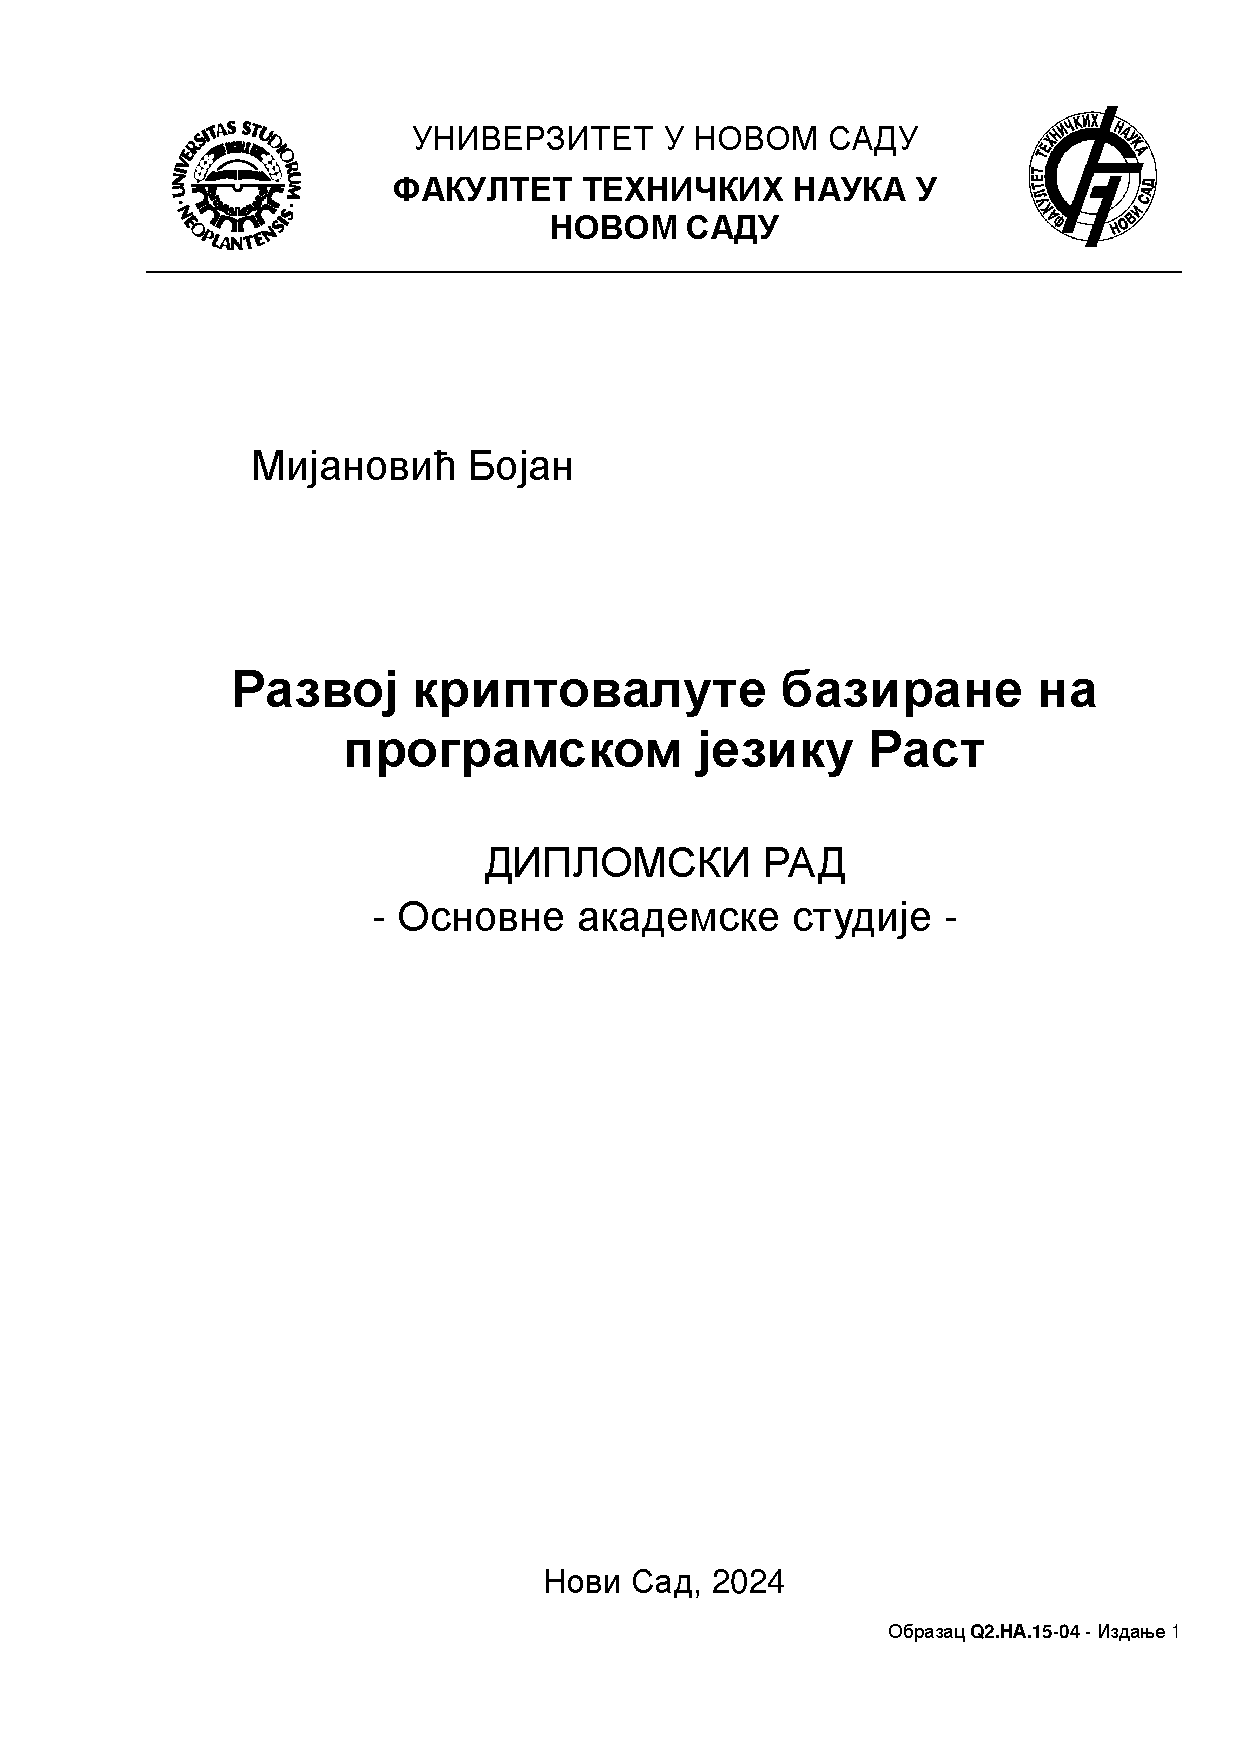
\includepdf[pages=-]{prva_strana.pdf}

\renewcommand{\contentsname}{Садржај}
\tableofcontents
\pagebreak

\section{Увод}
\textit{Blockchain} технологија представља дистрибутивну, децентрализовану и јавну базу свих трансакција \cite{1}.


Први концепт \textit{blockchain} технологије помиње се у 1982. години, када је Давид Чаум у својој дисертацији описао дистрибуирану базу података која користи криптографију \cite{2}. Овај рани рад није био директно повезан са дигиталним валутама, али је поставио темеље за будући развој \textit{blockchain} - а.

Права револуција долази 2008. године када Сатоши Накамото објављује рад "\textit{Bitcoin}: \textit{Peer-to-peer} електронски готовински систем", уводећи први модерни \textit{blockchain} и криптовалуту \textit{Bitcoin}. Генесис блок, први блок \textit{Bitcoin blockchain} - а, ископан је 3. јануара 2009. године, означавајући почетак \textit{blockchain} технологије какву данас познајемо \cite{3}.

\textit{Etherium}, лансиран 2015. године од стране Виталика Бутерина, увео је паметне уговоре који омогућавају сложеније трансакције и аутоматизацију различитих процеса. Овај развој проширио је примену \textit{blockchain} технологије далеко изван дигиталних валута, омогућавајући креирање децентрализованих апликација \cite{4}.

\textit{Blockchain} технологије су се од свог настанка имплементирале у различитим програмским језицима и окружењима. У својим раним фазама, \textit{blockchain} технологије су се углавном развијале користећи језике као што су \textit{C++} и \textit{Java}, захваљујући њиховој ефикасности и широкој употреби у индустрији. Касније, с појавом паметних уговора, \textit{Solidity} је постао стандард за развој на \textit{Etherium} платформи.

Овај рад се фокусира на имплементацију основних концепата \textit{blockchain} технологије у програмском језику \textit{Rust}, који је познат по својој сигурности, перформансама и могућности превенције грешака при руковању меморијом.

Рад је структуиран X целина
\pagebreak

\section{Основе \textit{Rust} програмског језика}
\textit{Rust} је савремени програмски језик који је развијен да буде безбедан и брз. Развијен од стране \textit{Mozilla Research}-а, \textit{Rust} је од свог настанка привукао велику пажњу због својих изузетних безбедносних карактеристика и перформанси \cite{5}.

\subsection{Увод у \textit{Rust} програмски језик}
\textit{Rust} је системски програмски језик, а уместо интерпретираног језика, као што су \textit{JavaScript} или \textit{Ruby}, има компајлер, као што имају \textit{Go}, \textit{C} или \textit{Swift}. Не комбинује активни \textit{runtime}, али обезбеђује језичку ергономију. Све је ово могуће захваљујући компајлеру који спречава грешке било којег типа и осигурава да не дође до проблема у меморији пре него што се покрене апликација \cite{6}.

\textit{Rust} обезбеђује перформансе (нема \textit{runtime}, нити прикупљање "смећа"), безбедност (компајлер осигурава да је све безбедно за меморију, чак и у асинхроним окружењима) и продуктивност (његове уграђене алатке за тестирање, документацију и "менаџер" пакета чине га лаким за израдз и одржавање) \cite{6}. 

\subsection{Зашто \textit{Rust} за \textit{blockchain}?}
Када је у питању развој blockchain апликација, \textit{Rust} се истиче као одличан избор из неколико разлога:
\begin{enumerate}
    \item \textbf{Безбедност меморије}: \textit{Rust}-ов систем власништва и провера за време компилације осигуравају да програмери избегну уобичајене грешке у раду са меморијом, што је критично за сигурност \textit{blockchain} система \cite{7}.
    \item \textbf{Перформансе}: \textit{Rust} је дизајниран да буде брз и ефикасан. Његов минималан \textit{overhead} и високо оптимизован компајлер резултирају брзим извршавањем кода, што је важно за обраду великог броја трансакција у реалном времену \cite{7}.
    \item \textbf{Паралелизам и конкурентност}: \textit{Rust} нуди снажну подршку за паралелно и конкурентно програмирање, омогућавајући оптимално коришћење мулти-језгарних процесора \cite{7}.
\end{enumerate}

\textit{Rust} нуди низ алата и библиотека које олакшавају развој сложених апликација. Две од најзначајнијих библиотека за развој \textit{blockchain} апликација су \textit{Tokio} и \textit{libp2p}. Ове библиотеке пружају подршку за асинхроне позиве и \textit{peer-to-peer} комуникацију, што је кључно за функционалност и ефикасност \textit{blockchain} система.

\pagebreak

% \textbf{\textit{Tokio}} је моћна асинхрона \textit{runtime} библиотека за \textit{Rust} која омогућава развој високоперформансних и високо доступних апликација. Кроз \textit{Tokio}, програмери могу да имплементирају асинхроне позиве и да развију веб сервере који могу да обрађују велики број истовремених веза.

Слика \ref{fig:2.1} прииказује технички стек који је укључен у одабир радног оквира. \textbf{\textit{Warp}} је довољно мали да се "склони са пута", довољно се користи да се њиме управља активно и има активну заједницу. Заснован је на \textit{Tokio runtime} - у. 


\begin{figure}[h]
    \centering
    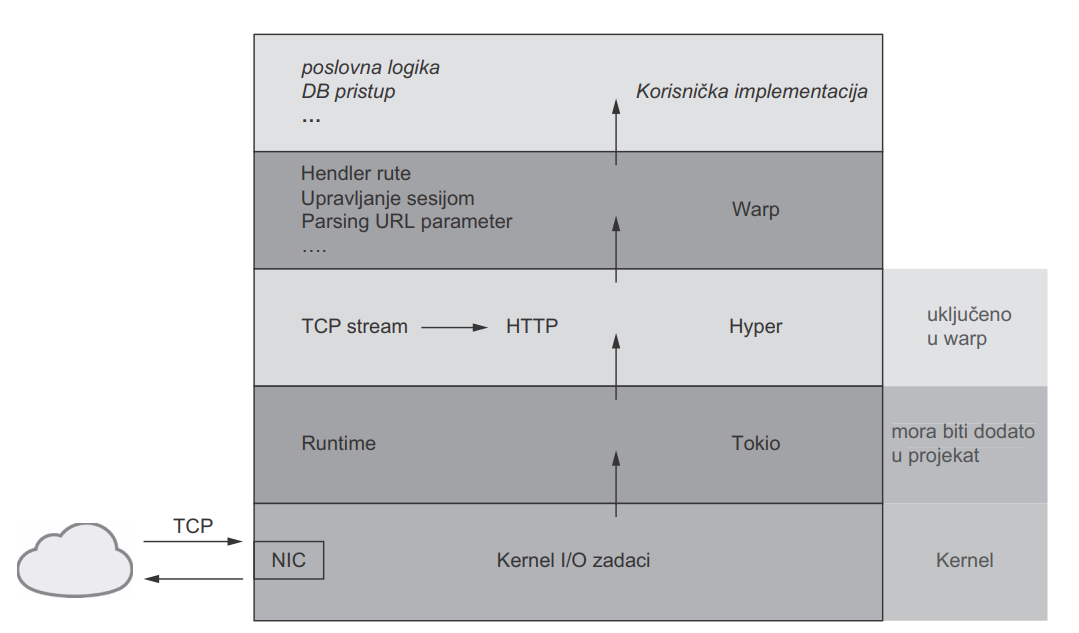
\includegraphics[width=1\linewidth]{slike/warp.png}
    \caption{\textit{Warp} веб радни оквир}
    \label{fig:2.1}
\end{figure}

\textit{\textbf{libp2p}} је модуларни мрежни стек који омогућава \textit{peer-to-peer} комуникацију. У контексту \textit{blockchain}-а, \textit{libp2p} се користи за омогућавање комуникације између различитих чворова у мрежи. Ова библиотека је флексибилна и подржава различите протоколе за пренос података, што је чини идеалном за развој децентрализованих апликација.

\pagebreak

\section{Увод у \textit{blockchain} технологију}
\textit{Blockchain} технологија представља савремен приступ складиштењу и дистрибуцији података. Основни принципи и концепти \textit{blockchain} технологије нуде дубоку промену у начину на који се информације похрањују, проверавају и дистрибуирају путем децентрализоване мреже рачунара.

\subsection{Основни принципи и концепти}
\textit{Blockchain} се може дефинисати као дистрибуисана дигитална књига трансакција. Основна идеја је стварање низа блокова који садрже податке. Блкови су криптографски повезани тако да је немогуће мењати податке у претходним блоковима без мењања свих следећих блокова \cite{8}. 

Кључни елементи \textit{blockchain}-а укључују:
\begin{enumerate}
    \item \textbf{Децентрализација}: Подаци се похрањују и управљају путем мреже чворова уместо централизованог ауторитета, што осигурава транспарентност и отпорност на цензуру.
    \item  \textbf{Дистрибуираност}: Сваки чвор у мрежи садржи комплетан или део \textit{blockchain}-а, омогућујући свима у мрежи да виде исте податке. Ово спречава појединачне тачке квара и повећава отпорност на нападе.
    \item \textbf{Сигурност}: Криптографски алгоритми осигуравају да је свака промена у \textit{blockchain}-у лако проверљива, а трансакције се потврђују кроз консензус мреже.
    \item \textbf{Неповратност}: Након што је трансакција забележена у \textit{blockchain}-у, тешко ју је променити или обрисати без сагласности већине чворова у мрежи, чиме се осигурава поверење и интегритет података.
\end{enumerate}


\subsection{Поређење са традиционалним базама података}
Насупрот традиционалним базама података које су често централизоване и ослањају се на поверење у једну јединицу, \textit{blockchain} нуди неколико кључних разлика:
\begin{enumerate}
    \item \textbf{Централизација у односу на децентрализацију}: Традиционалне базе података често су централизоване под контролом једне организације. \textit{Blockchain} дистрибуише податке широм мреже, елиминишући потребу за централним ауторитетом.
    \item \textbf{Транспарентност и проверљивост}: \textit{Blockchain} омогућава свим корисницима увид у све трансакције које су се догодиле, што повећава транспарентност и смањује могућност манипулације.
    \item \textbf{Сигурност и отпорност}: Због своје дистрибуиране природе, \textit{blockchain} је отпорнији на нападе и кварове у поређењу са традиционалним базама података које су осетљиве на појединачне тачке квара.
    \item \textbf{Ефикасност и трошкови}: Иако \textit{blockchain} може бити спорији у обради података у поређењу са централизованим базама података, његова сигурност и транспарентност могу надмашити трошкове и ризике традиционалних система.
\end{enumerate}

\newpage
\section{Архитектура апликације}
\textit{Blockchain} технологија се састоји од неколико кључних компоненти које омогућавају њено функционисање. Основне јединице података су блокови, који садрже информације о трансакцијама, временским ознакама и криптографским хеш функцијама претходних блокова. Ови блокови су повезани у секвенцијални ланац, познат као \textit{blockchain}, који осигурава неповредивост података. 

Дистрибуирана мрежа чворова заједнички одржава и верификује \textit{blockchain}, омогућавајући децентрализацију. Консензус алгоритми, као што су \textit{Proof of Work (PoW)} и \textit{Proof of Stake (PoS)}, омогућавају учесницима мреже да се сложе око валидности нових блокова. Криптографија осигурава сигурност и приватност података унутар \textit{blockchain} -а, користећи хеш функције и дигиталне потписе. 

У наредним подсецијама, детаљно ћемо описати сваку од ових компоненти, укључујући процесе као што су PoW и мајнинг, који су кључни за додавање нових блокова у ланац.


\subsection{Блокови}
Блокови су основне јединице података у \textit{blockchain} технологији. Сваки блок садржи скуп података који су повезани са трансакцијама и другим важним информацијама. У контексту \textit{blockchain}-а, блокови су организовани у ланац, где сваки блок садржи хеш претходног блока, што обезбеђује интегритет и сигурност података. Следећи код приказује структуру блока у Rust програмском језику:

\begin{minted}{rust}
pub struct Block {
    pub timestamp: DateTime<Utc>,
    pub last_hash: String,
    pub hash: String,
    pub data: Vec<Transaction>,
    pub nonce: u64,
    pub difficulty: u64,
}
\end{minted}

Атрибути блока су:
\begin{itemize}
    \item \textbf{timestamp}: Време када је блок креиран. Овај атрибут омогућава праћење хронологије трансакција у \textit{blockchain}-у.
    \item \textbf{last\_hash}: Хеш вредност претходног блока у ланцу. Овај атрибут обезбеђује да сваки блок буде повезан са својим претходником, чиме се осигурава интегритет ланца.
    \item \textbf{hash}: Хеш вредност тренутног блока. Ова вредност се добија применом хеш функције на садржај блока и служи као јединствени идентификатор блока.
    \item \textbf{data}: Податке у блоку, који обично укључују трансакције. У овом случају, то је вектор трансакција \textit{(Vec<Transaction>)}.
    \item \textbf{nonce}: Произвољни број који рудари мењају током процеса рударења како би добили хеш вредност блока која задовољава критеријуме тешкоће.
    \item \textbf{difficulty}: Ниво тежине који одређује колико је сложено пронаћи важећи хеш за блок. Тежина рударења се прилагођава да би се одржала константна брзина креирања блокова у мрежи.
\end{itemize}



\subsubsection{Генесис блок}
Генесис блок је први блок у ланцу блокова и служи као темељ целокупног \textit{blockchain} система (Слика \ref{fig:genesis-block}). Он нема претходника и обично је ручно креиран од стране креатора \textit{blockchain}-а. Генесис блок обично садржи посебне параметре и почетне вредности које су специфичне за дат \textit{blockchain}. Његова важност лежи у чињеници да сваки наредни блок у ланцу зависи од њега кроз хеш вредности.

\begin{figure}[h]
    \centering
    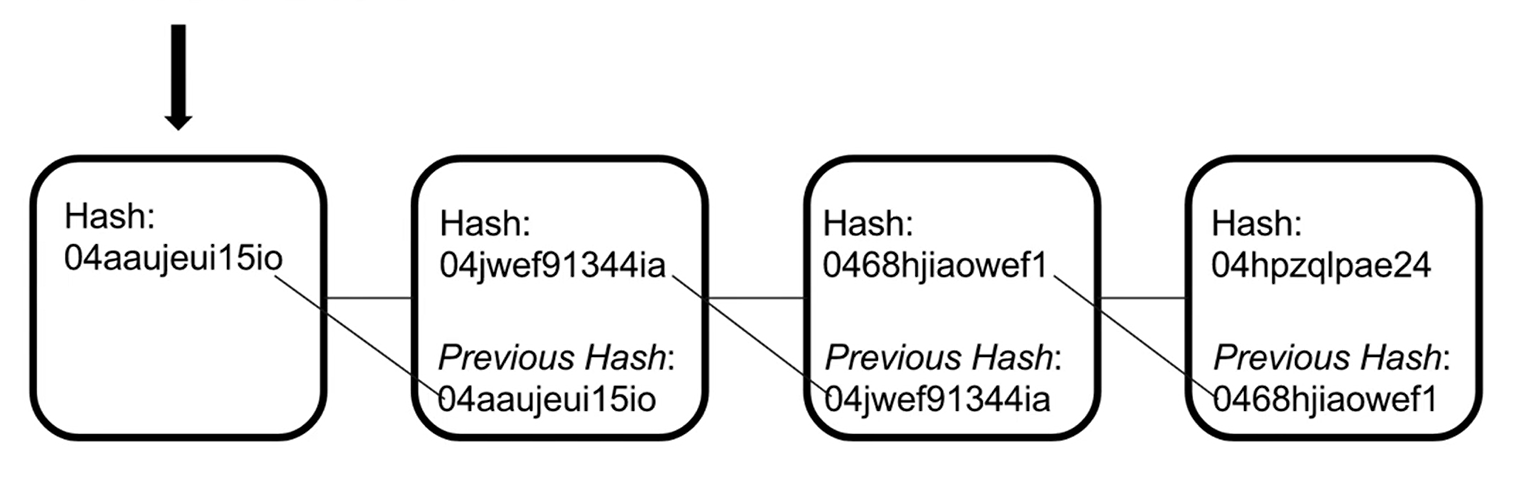
\includegraphics[width=1\linewidth]{slike/genesis.png}
    \caption{Приказ генесис блока у \textit{blockchain}-у}
    \label{fig:genesis-block}
\end{figure}

\subsubsection{Рударење}
Рударење је процес додавања нових блокова у \textit{blockchain}. Рудари користе своју рачунарску снагу да реше комплексне математичке проблеме који су потребни за валидацију нових трансакција и креирање нових блокова. Овај процес захтева значајну количину енергије и ресурса, али је кључан за одржавање безбедности и децентрализације \textit{blockchain} мреже. У процесу рударења, рудари се такмиче да пронађу одговарајући \textit{nonce} који ће произвести хеш вредност која испуњава одређене критеријуме тешкоће.


\subsubsection{Хеш функција}
Хеш функција је критичан елемент у \textit{blockchain} технологији, јер обезбеђује сигурност и интегритет података у блоковима. Хеш функција узима улазне податке произвољне дужине и генерише фиксну дужину излазне вредности, која је јединствена за те улазне податке. У контексту \textit{blockchain}-а, хеш функција се користи да повезује сваки блок са претходним блоком, чиме се обезбеђује да свака промена у подацима било ког блока одмах утиче на све наредне блокове, што чини \textit{blockchain} изузетно отпорним на манипулацију.



\subsection{Ланац}
\textit{Blockchain} је структура података која се састоји од низа повезаних блокова, где сваки блок садржи хеш претходног блока, чиме се обезбеђује интегритет и сигурност ланца. Следећи код приказује структуру \textit{blockchain}-а у \textit{Rust} програмском језику:

\begin{minted}{rust}
pub struct Blockchain {
    pub chain: Vec<Block>,
}
\end{minted}

Атрибут \textit{\textbf{chain}} је вектор који чува редоследно повезане блокове, формирајући ланац блокова.
Слика \ref{fig:genesis-blockchain} приказује структуру ланца са генесис блоком на почетку.
\begin{figure}[h]
    \centering
    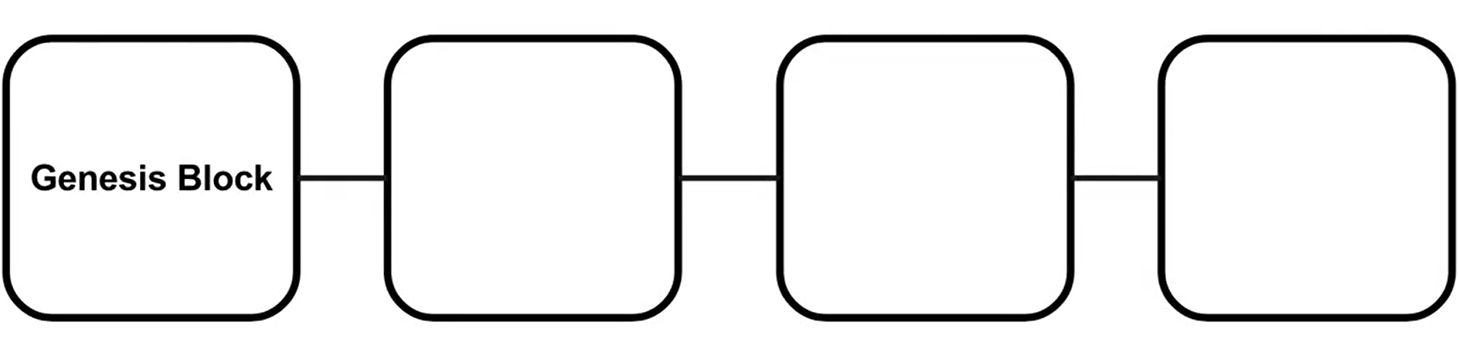
\includegraphics[width=1\linewidth]{slike/blockchain.png}
    \caption{Приказ идеје \textit{blockchain}-a}
    \label{fig:genesis-blockchain}
\end{figure}

\newpage
\subsubsection{Валидација више ланаца}
Идеја овог механизма је да подржи више доприносиоца, при чему ће више доприносиоца додавати блокове у \textit{blockchain}. Сваки рудар ће имати своју верзију истог ланца. Када један рудар дода нови блок у ланац, мораће да пошаље тај нови блок осталим ланцима у систему како би они прихватили ту промену и ажурирали целокупни систем. На тај начин сви добијају ажурирану копију са тим новим блоком, чиме се осигурава да сви ланци буду конзистентни.


\begin{figure}[h]
    \centering
    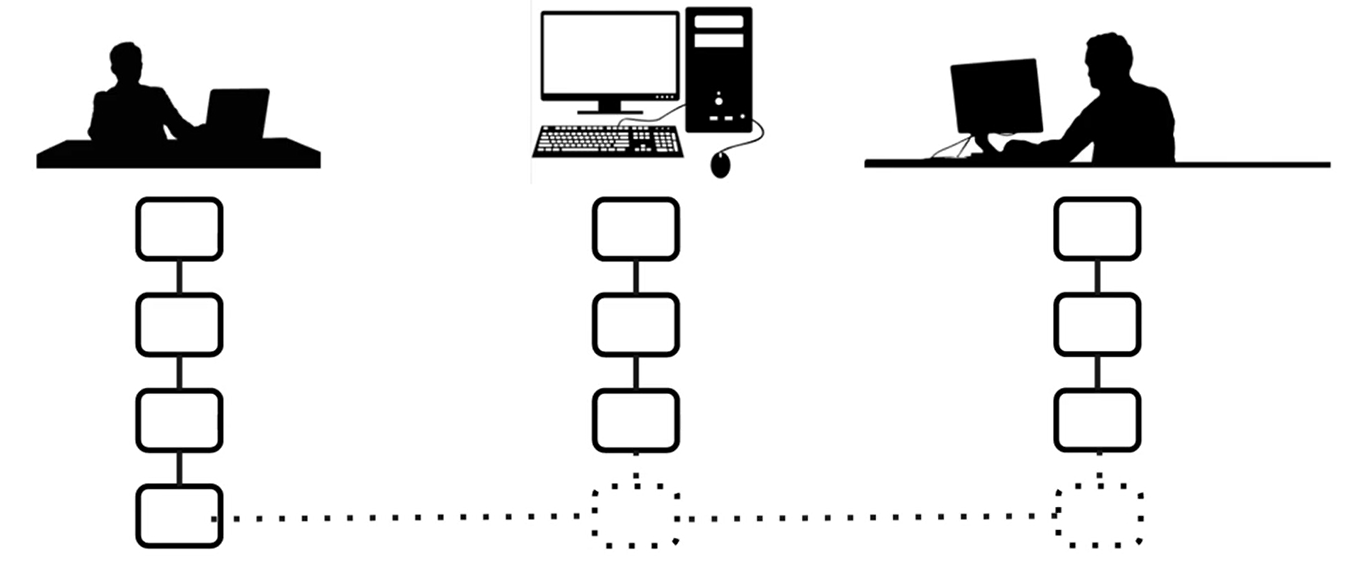
\includegraphics[width=1\linewidth]{slike/multiple-chain-validation.png}
    \caption{Приказ дељења ланаца}
    \label{fig:multiple-chain-validation}
\end{figure}

Међутим, да би сви рудари прихватили ове нове ланце, мора постојати неки облик валидације који ће осигурати да је нови блок валидан и да треба да буде прихваћен. Главни облик валидације је прихватање дужих ланаца који стигну. На пример, ако сви имају договорени \textit{blockchain} који је већ дуг три блока, и један рудар дода два блока у ланац, док други рудар дода само један блок у исто време, систем ће прихватити дужи ланац. На тај начин се осигурава да договорени ланац за све увек буде онај који садржи највише података.


\begin{figure}[h]
    \centering
    \begin{minipage}{0.45\linewidth}
        \centering
        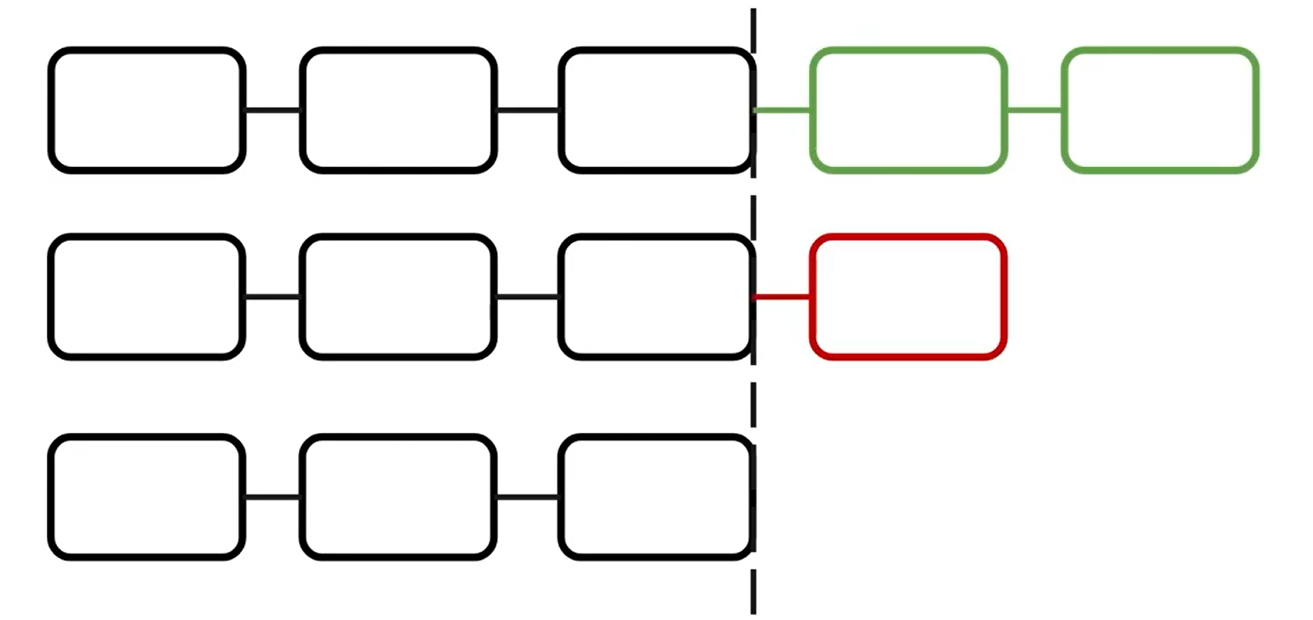
\includegraphics[width=\linewidth]{slike/longer-chains-before.png}
        \caption{Стање пре валидације}
        \label{fig:validation-1}
    \end{minipage}
    \hfill
    \begin{minipage}{0.45\linewidth}
        \centering
        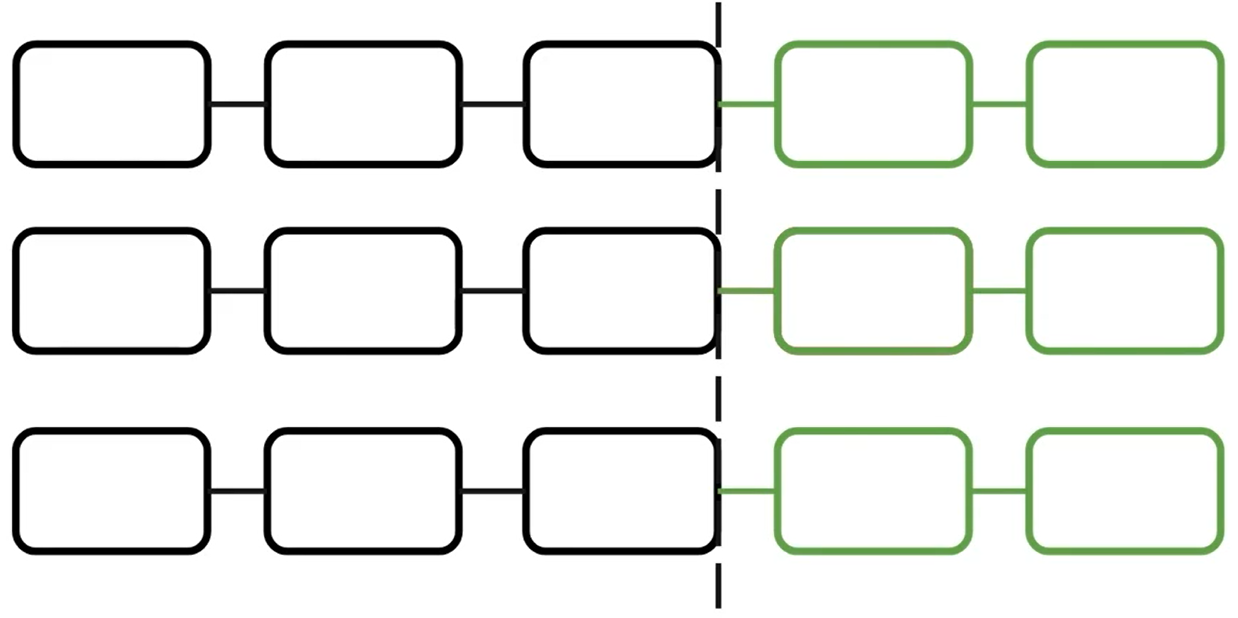
\includegraphics[width=\linewidth]{slike/longer-chains-after.png}
        \caption{Стање после валидације}
        \label{fig:validation-2}
    \end{minipage}
\end{figure}

\newpage
Ово такође решава проблем рачвања у ланцу. На пример, ако две одвојене инстанце \textit{blockchain}-а истовремено произведу један блок на основу претходног блока, настаје рачвање у систему где оба рудара производе блок на основу истог претходног блока (слика \ref{fig:forks-a}). Пола рудара ће имати ланац који је произвео рудар А, а друга половина ће имати ланац који је произвео рудар Б (слика \ref{fig:forks-b}). Коначно, систем треба да дође до договора о томе који ланац ће прихватити. Ако неко дода неколико блокова на ланац рудара А, тај ланац ће сада бити дужи од свих осталих у систему (слика \ref{fig:forks-c}). Сви ће морати да прихвате најдужи ланац, који садржи блок од рудара А, чиме се решава рачвање прихватањем оригиналног блока од рудара А (слика \ref{fig:forks-d}).

\begin{figure}[h]
    \centering
    \begin{subfigure}{0.45\linewidth}
        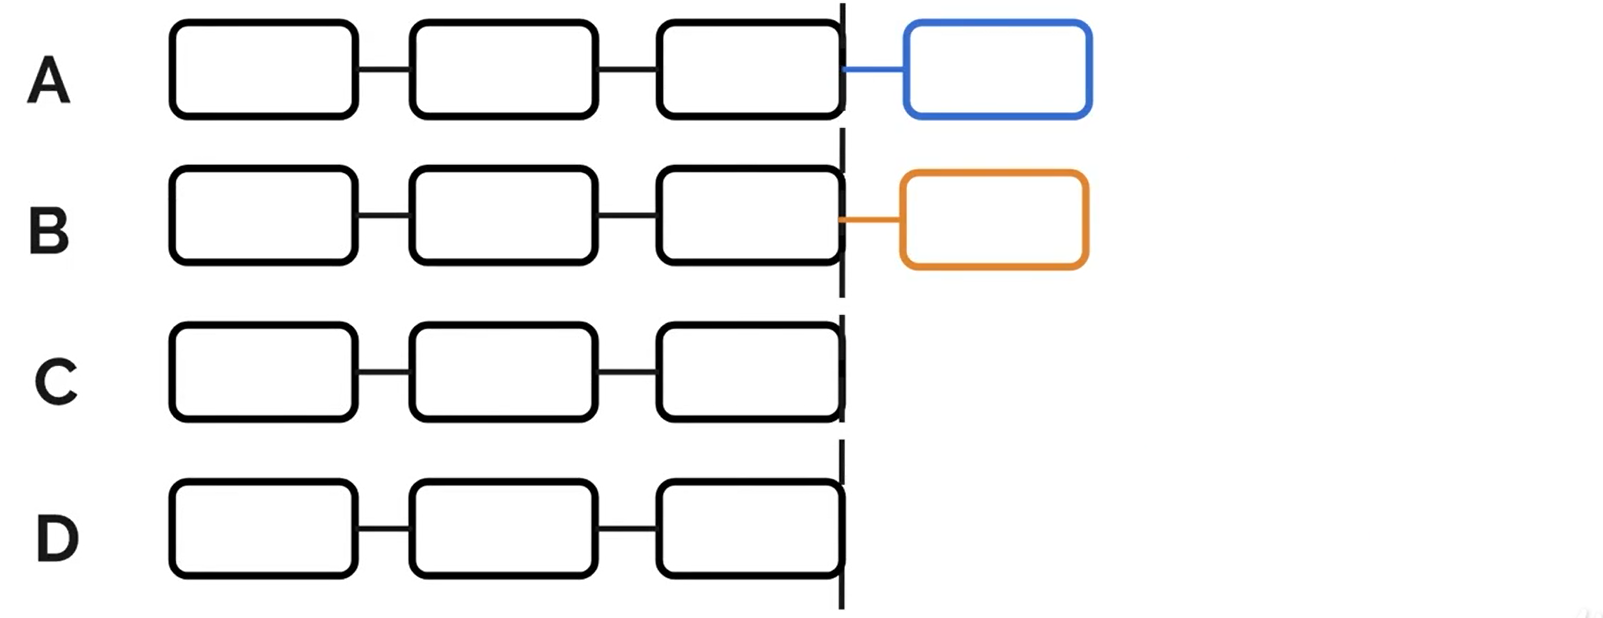
\includegraphics[width=\linewidth]{slike/forks-1.png}
        \caption{Додавање различитих блокова}
        \label{fig:forks-a}
    \end{subfigure}
    \hfill
    \begin{subfigure}{0.45\linewidth}
        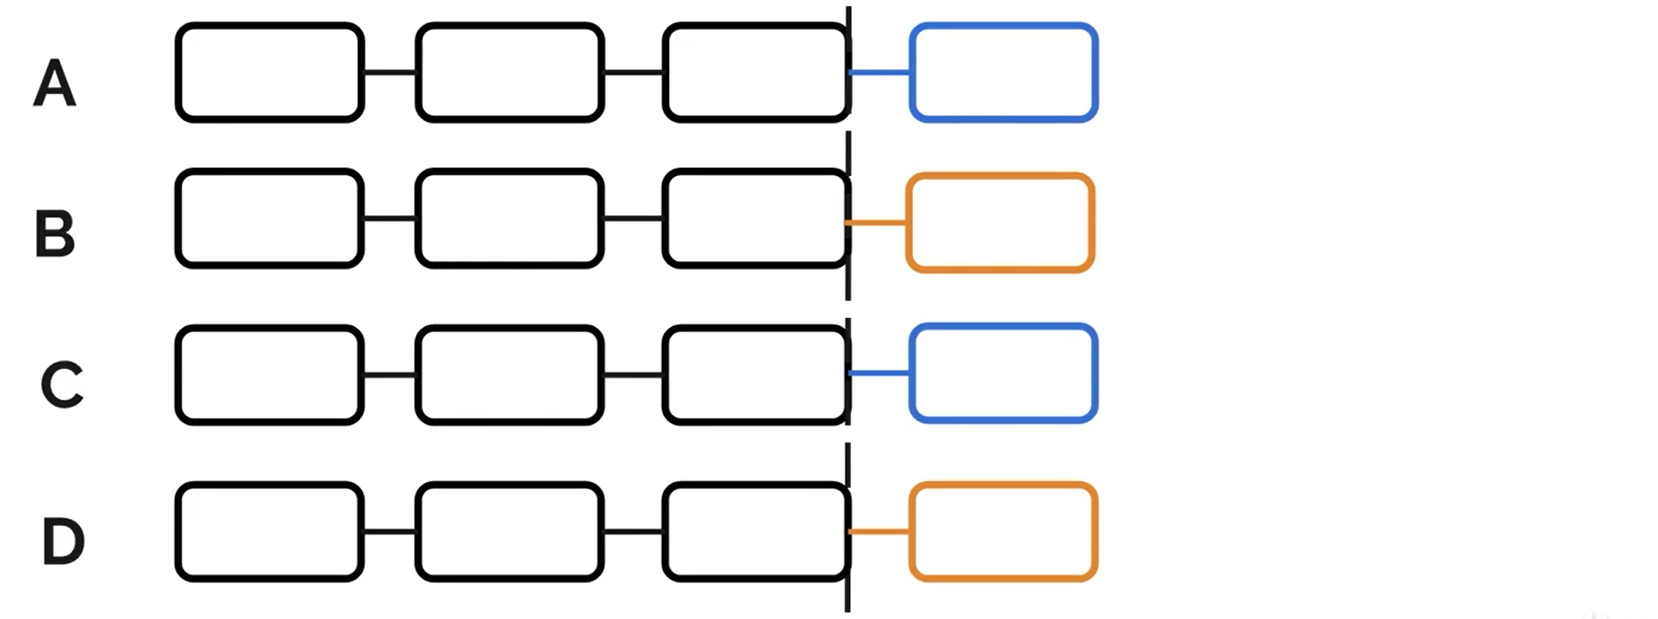
\includegraphics[width=\linewidth]{slike/forks-2.png}
        \caption{Размена различитих ланаца}
        \label{fig:forks-b}
    \end{subfigure}

    \begin{subfigure}{0.45\linewidth}
        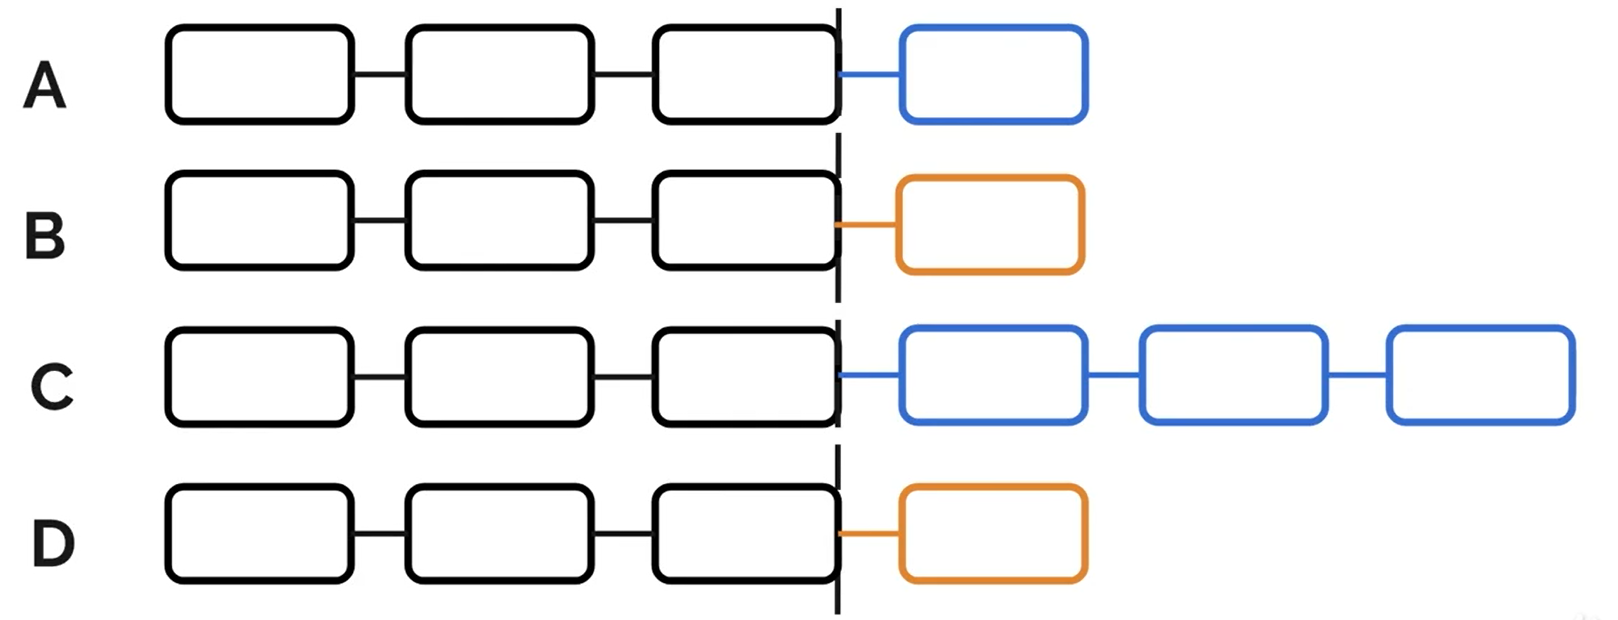
\includegraphics[width=\linewidth]{slike/forks-3.png}
        \caption{Додавање нових блокова}
        \label{fig:forks-c}
    \end{subfigure}
    \hfill
    \begin{subfigure}{0.45\linewidth}
        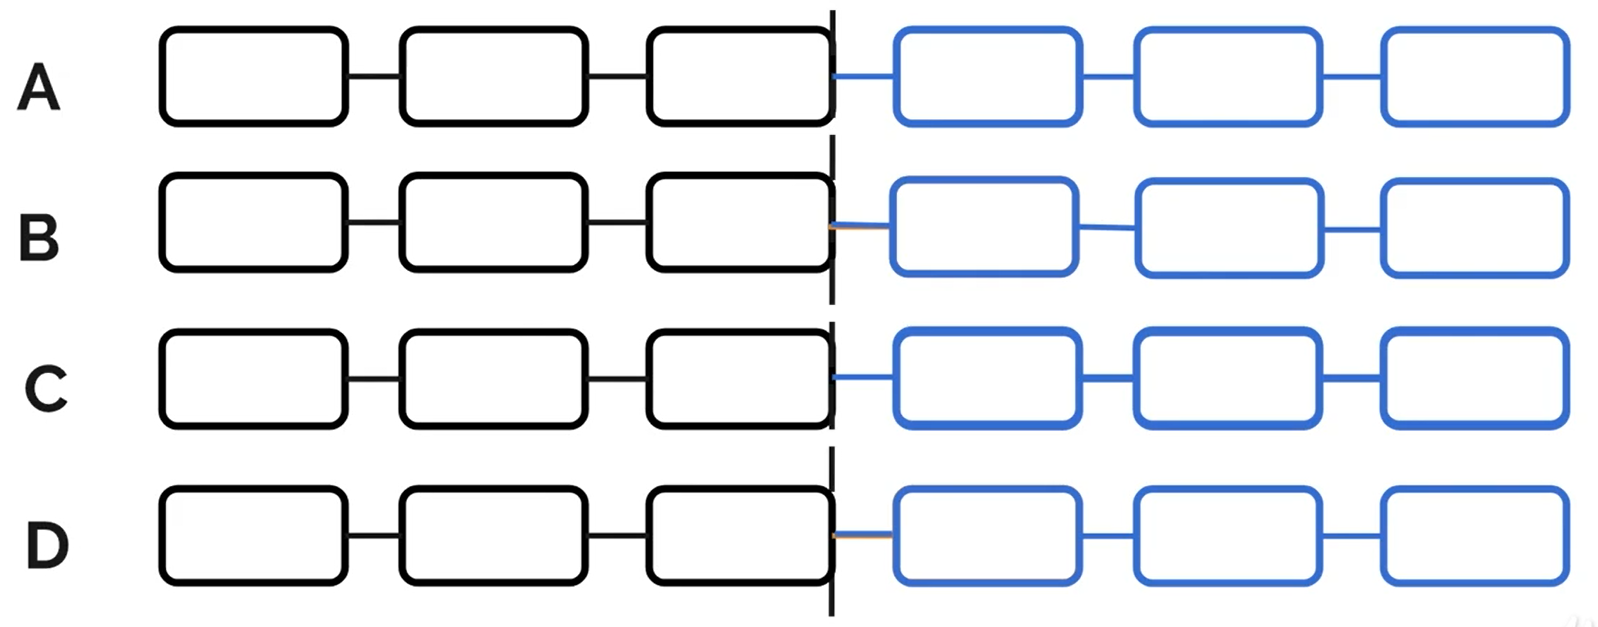
\includegraphics[width=\linewidth]{slike/forks-4.png}
        \caption{Прихватање најдужег ланца}
        \label{fig:forks-d}
    \end{subfigure}
    \caption{Решавање рачвања}
    \label{fig:combined}
\end{figure}

Ово не значи да блокови са ланца рудара Б губе оригиналне податке, јер се блок који није укључен у рачвање може сада додати на крај новоприхваћеног ланца.

Други облик валидације је провера вредности хеша произведених за сваки блок ланца. Сваки \textit{blockchain} има приступ хеш функцији која генерише хеш на основу података блока. Када \textit{blockchain} прими нови ланац, може осигурати да је хеш исправно генерисан тако што ће сам поново генерисати тај хеш. Ако се хешеви не поклапају, вероватно су подаци мењани, и због тога \textit{blockchain} неће прихватити нови ланац.


\subsection{\textit{Proof of work}}
\textit{Proof of work} систем је систем који захтева од рударa да троше време на рачунарски рад како би додали блокове у ланац. Ово има корист у одвраћању неискрених учесника од замене \textit{blockchain}-а корумпираним и неважећим подацима.

Да би се објаснило како се неискрени чворови одвраћају, треба узети у обзир да у децентрализованом \textit{blockchain}-у сваки чвор има могућност подношења новог ланца систему. Све док је тај ланац довољно дуг и садржи важеће хеш податке, почевши од генезис блока, тај ланац ће бити прихваћен од свих чворова у мрежи \textit{blockchain}-а.

Међутим, како би се одвратили неискрени појединци у мрежи од преузимања целог \textit{blockchain}-а са корумпираним ланцем у њихову корист, који заправо има важеће хешеве, систем доказивања рада чини то рачунарски скупим.

\textit{Proof of work} систем чини да појединачни чворови у \textit{blockchain}-y морају уложити велику количину рачунарског рада како би додали блок. Међутим, за неискрене чворове, доказивање рада чини веома непродуктивним покушај преузимања са потпуно ново генерисаним ланцем.

\textit{Proof of work} систем функционише на следећи начин. У сваком тренутку постоји ниво тежине у систему \textit{blockchain}-а. У зависности од ове тежине, неко ко покушава да дода нови блок мора пронаћи хеш вредност за тај блок која одговара овој тежини. За ово поклапање, рудари морају пронаћи исти број водећих нула као што је тренутна тежина за генерисани хеш новог блока који треба додати у ланац.

\begin{figure}[h]
    \centering
    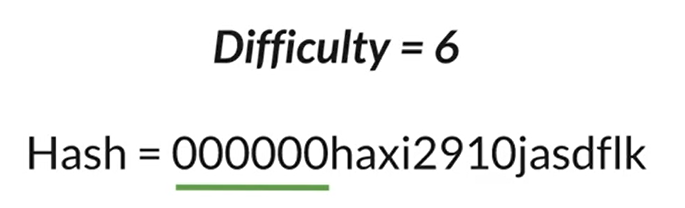
\includegraphics[width=0.5\linewidth]{slike/difficulty.png}
    \caption{Приказ задовољеног хеша}
    \label{fig:good-hash}
\end{figure}

Пронаћи одређени број водећих нула насумично постаје експоненцијално теже како се сама тежина повећава. Дакле, да би се решио доказ рада, рудар ће морати генерисати огроман број хешева како би на крају пронашао један који задовољава тежину. Они ће генерисати нове хешеве за исти блок на основу података блока као и његове прилагођене вредности зване \textit{nonce}.

\subsubsection{\textit{Nonce}}
Променом вредности нонса рудар генерише нове важеће хешеве за текући блок и његове податке. \textit{Nonce} је термин у криптографији који се односи на вредност која се може користити само једном. Пошто свака јединствена вредност \textit{nonce}-a генерише јединствен хеш, \textit{nonce}-i се могу користити само једном за генерисање тог новог хеша за блок.

Вредност нонса почиње од нуле и повећава се док се не пронађе \textit{nonce} који има одговарајући број водећих нула у складу са подешеном тежином, што генерише хеш. Ова вредност \textit{nonce}-a се затим чува као део блока.

\subsubsection{Процес рударења}
Овај процес генерисања нових хешева са променљивим вредностима захтева доста рачунарског рада. Због тога се акт трошења овог рачунарског рада назива рударење. Када рудар успешно ископа блок, они ће поднети свој блок са пронађеном вредношћу нонса осталим рударима.

Када остали рудари сазнају ову вредност нонса, они могу брзо проверити ваљаност тог решења и додати нови блок у ланац. На тај начин, они не морају поново да раде исти рачунарски рад када приме нови блок за додавање у свој \textit{blockchain} и остану ажурни.

\subsubsection{Динамичка тежина додавања блокова}
Са вредношћу \textit{nonce}-a у блоку, имплементирали смо \textit{Proof of work} систем, где рудари морају уложити одређену количину рачунарске снаге како би додали блокове у ланац. Међутим, како се у мрежу \textit{blockchain}-а додаје све више учесника, блокови ће се откривати брже, јер ће постојати већа шанса да бар један рудар пронађе валидан хеш при одређеној тежини. Због тога нам је потребан динамичан систем који прилагођава ниво тежине \textit{blockchain}-а како се у систем додаје све више рудара.

Да бисмо то постигли, можемо додати вредност тежине сваком блоку. Поред тога, такође постављамо временску вредност која представља стопу којом желимо да се сваки блок рудари. Механизам за прилагођавање тежине функционисаће на следећи начин: проверићемо временски жиг ново изрудареног блока и упоредити га са временским жигом претходно изрудареног блока. Ако је разлика између оба временска жига мања од постављене стопе рударења, знамо да је блок изрударен сувише брзо, те ће се тежина повећати за 1. Слично томе, ако је разлика у временским жиговима између нашег најновијег блока и блока који је претходио већа од стопе рударења, знамо да је блок изрударен сувише споро, те ће се тежина смањити за 1. Са овим системом, увек ћемо прилагођавати тежину за сваки блок и требао би имати систем који рудари блокове у одређеним интервалима.


\begin{figure}[h]
    \centering
    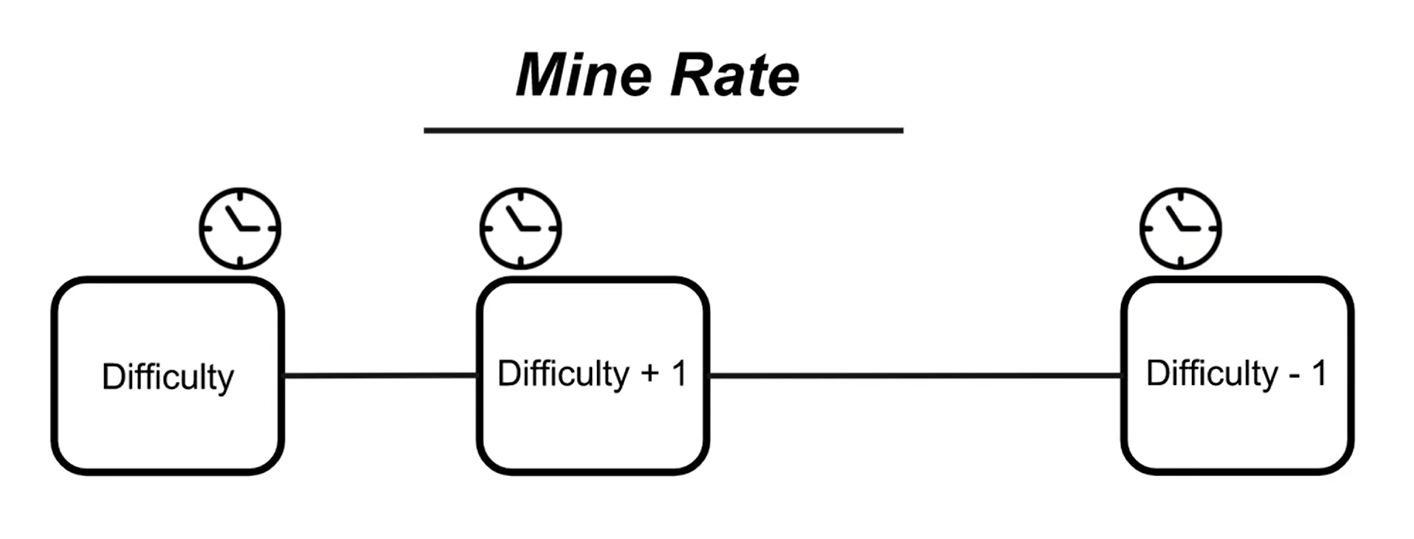
\includegraphics[width=0.7\linewidth]{slike/dynamic-block-difficulty.png}
    \caption{Динамичка промена тежине рударења блока}
    \label{fig:dynamic-mine-rate}
\end{figure}



% \subsection{Новчаник и трансакције}
% \subsubsection{Новчаник}
% \subsubsection{Креирање кључева}
% \subsubsection{Трансакције}
% \subsubsection{Потписивање трансакција}
% \subsubsection{Верификација трансакција}
% \subsubsection{Ажурирање трансакција}

% \subsection{Базен трансакција}

% \subsection{Рудари}
% \subsubsection{Добављање валидне трансакције}
% \subsubsection{Наградне трансакције}
% \subsubsection{Пражњење базена трансакција}
% \subsubsection{Стање новчаника}

% \section{\textit{HTTP} сервер}
% \section{\textit{P2P} сервер}
% \section{Ограничења и унапређења}
% \section{Закључак}



\pagebreak
\section{Литература}
\renewcommand{\refname}{}
\vspace{-\parskip} % Remove extra space added by \parskips
\vspace{-\parskip} % Remove extra space added by \parskips
\vspace{-\parskip} % Remove extra space added by \parskips
\vspace{-\parskip} % Remove extra space added by \parskips
\bibliography{bibliography}


\pagebreak
\section{Подаци о кандидату}
Кандидат Бојан Мијановић је рођен 2002. године у Зрењанину. Завршио је средњу школу у Зрењанину, 2020. године као ђак генерације. Факултет Техничких Наука у Новом Саду је уписао 2020. године. Испунио је све обавезе и положио је све испите предвиђеним студијским програмом са просечном оценом од 9.75.


\end{document}

